\documentclass[12pt,a4paper,hidelinks]{report}
\usepackage[margin=0.75in]{geometry}
\usepackage{parskip}
\usepackage{fontspec}
\usepackage{titling}
\usepackage{amsmath, amsthm, amssymb}
\usepackage{hyperref}
\usepackage{graphicx}
\usepackage{caption}

\setmainfont{Times New Roman}

\title{\Huge{Pixel Hackenbush}}
\date{\today}
\author{Seyed Mohammad Ghazanfari}
\begin{document}
\linespread{1.15}\selectfont
\maketitle

\tableofcontents

\begin{abstract}
  This repository contains a simple yet engaging implementation of the Hackenbush game, built using the Flutter framework and the Flame game engine. It's designed to be both fun and easy to play, leveraging the capabilities of Flutter for cross-platform compatibility and Flame for a smooth gaming experience~\footnote{Clone this project from \href{https://github.com/mgh5225/pixel_hackenbush}{here}.}.
\end{abstract}

\chapter{Introduction}

Hackenbush is a combinatorial game with a set of rules and strategies that can be analyzed mathematically. The game is played on a drawn figure consisting of vertices and line segments connected to a base line called the ground. Players alternate turns, removing a line of their color—blue for the Left player and red for the Right player. When a line is disconnected from the ground, it and any lines depending on it are removed. Since this game is normal-play, the last player to make a move wins~\cite{game-theory}.
\par
To understand more general positions in this game (like nimbers in Nim), We assign numbers to certain Hackenbush positions. We have the following equation for every Hackenbush position $\alpha$:

\begin{equation}
  \alpha + \bullet\text{0} \; \equiv \; \alpha
\end{equation}

$\bullet\text{0}$ is defined to be the Hackenbush position with no edges (so there are no available moves). The position $\bullet\text{0}$ is type $P$.
If $\alpha$ and $\beta$ are Hackenbush positions, then


\begin{align}
  -(-\alpha) \; \equiv \;         & \alpha                                                         \\
  \alpha + (-\alpha) \; \equiv \; & \bullet\text{0}                                                \\
  \beta + (-\alpha) \; \equiv \;  & \bullet\text{0} \; \text{implies} \; \alpha \; \equiv \; \beta
\end{align}

For every positive integer $n$, define $\bullet n$ to be the Hackenbush position consisting of $n$ isolated blue edges. For a negative integer $-m$, we define $\bullet (-m)$ to be the Hackenbush position consisting of $m$ isolated red edges. We may view $\bullet$ as an operation that takes an integer and outputs a special kind of Hackenbush position.
For any integers $m$ and $n$, we have

\begin{align}
  - (\bullet n) \; \equiv \;             & \bullet (-n)  \\
  (\bullet m) + (\bullet n) \; \equiv \; & \bullet (m+n)
\end{align}

It is straightforward to determine the type of an Hackenbush position since in each such position some player has no moves.

\begin{equation}
  \text{Type of position $\bullet n$ is}
  \begin{cases}
    L & n > 0, \\
    P & n = 0, \\
    R & n < 0.
  \end{cases}
\end{equation}

We talked all about integer positions like $\bullet n$. Could there be a Hackenbush position $\alpha$ that gives a player an advantage of $\frac{1}{2}$? The answer is Yes! For every positive integer $k$, we have $\bullet \frac{1}{2^k} + \bullet \frac{1}{2^k} \; \equiv \; \bullet \frac{1}{2^{k-1}}$.
\par
To generalize rules we talked about earlier, we turn to a special kinds of numbers called \textit{Dyadic Numbers}. Any number that can be expressed as a fraction where the denominator is a power of 2 (and the numerator is an integer) is called a dyadic number. For example, $\frac{17}{32}$ and $\frac{531}{64}$ are dyadic numbers, but $\frac{2}{7}$ and $\pi$ are not. It is obvious that any integer numbers are dyadic numbers (the denominator can be one or $2^0$).
\par
As every dyadic number has a unique (finite) binary expansion (can be proved), for every dyadic number $q > 0$ with binary expansion $2^{d_1} + 2^{d_2} + \dots + 2^{d_l}$ (here $d_1 > d_2 > \dots > d_l$ are integers which may be positive), we define the Hackenbush position $\bullet q$ as follows:

\begin{equation}
  \bullet q = \bullet 2^{d_1} + \bullet 2^{d_2} + \dots + \bullet 2^{d_l}
\end{equation}

\chapter{Game Assets}

The game's assets originate from external sources. To build and execute the project, you must independently acquire these assets by consulting the provided reference~\cite{assets}.

To utilize the images within the project, a conversion process is required where multiple images are combined into a single composite image. For instance, the main character's idle animation is composed of five separate images, each measuring $60\times40$. These should be merged horizontally to form a composite image with dimensions $320\times40$. Once you've transformed each set of animation frames into a single image, place them in the \verb|assets/images| directory, ensuring they are sorted into the appropriate subdirectories. As an example, the main character's animations would be located in \verb|assets/images/Character|.

To build and create a level for this project \textit{Tiled Map Editor} is used. You can access this application by referring to~\cite{tiled}.

\chapter{Gameplay}

\section{Menus}

In this project, all menus are developed using the Tiled application. Each menu can be viewed in Appendix~\ref{appendix:images}.
The design process is modular, allowing for the creation of complex menus using different properties. In other words, different properties are set to create complex menus using \verb|flutter| and \verb|flame_tiled| packages. For instance, you can create a button with different functionalities and types like icon button, toggle button, and more.
\par
The \verb|flame_tiled| package serves as a bridge between the Flame game engine and Tiled maps. It parses TMX (XML) files and accesses the tiles, objects, and other elements within them.

\section{Player}

In a game, each player is characterized by a 2D vector representing their velocity. This vector (x, y) indicates the direction in which the player can move. The game reads inputs from the keyboard, such as pressing arrow keys, enter, or space bar, and acts accordingly.
\par
The game continuously checks the current state of the player and updates it if necessary. This could involve changing the player's velocity if they press an arrow key, updating the player's animation, like if they start or stop running.

\section{Physics}

Figure~\ref{fig:collisions} illustrates that each game object, including the player, walls, and ground, is represented by a rectangle box. The player class incorporates a \verb|CollisionCallbacks| mixin, enabling the player to listen for collisions. Upon collision with another game object, the type of the object is assessed (e.g., \verb|CollisionBlockType.platform|, and \verb|CollisionBlockType.ground|), and actions are taken accordingly. Four methods are designed to determine the direction of the collision relative to the player.
\par
To determine the collision direction, we calculate the normal vector between the player's position and the midpoint of two intersection points. This vector is then multiplied by predetermined vectors representing the four cardinal directions (\verb|fromTop|, \verb|fromBottom|, \verb|fromLeft|, and \verb|fromRight|). If the resulting value exceeds a certain threshold, the method returns \verb|true|, indicating a collision in that direction. Otherwise, the player is not colliding with the object in that direction. Additional conditions ensure the player is colliding in a specific direction.

\section{Interaction With Objects}

In this modified version of the Hackenbush game, there are three players, each with the ability to attack a designated enemy:

\begin{itemize}
  \item Player one can attack 
\includegraphics[height=\fontcharht\font`\B]{assets/enemy-1.png}
  \item Player two can target 
\includegraphics[height=\fontcharht\font`\B]{assets/enemy-2.png}
  \item Player three is assigned to attack 
\includegraphics[height=\fontcharht\font`\B]{assets/enemy-3.png}
\end{itemize}

Each player has a unique adversary and cannot attack enemies assigned to others. In Figure~\ref{fig:enemies} we can see an example of these enemies on top of each other.
\par
When the player presses the attack button, a raycast is initiated from the player's forward direction to determine if an enemy is in range. If the raycast collides with an enemy that is compatible with the player's attack, that enemy and any additional enemies stacked with it are eliminated, in accordance with the Hackenbush game rules.

\appendix

\chapter{Assets Structure}

The directory structure for \verb|assets/images| should be organized as follows:

\begin{verbatim}
  Backgrounds
    Additional Sky.png
    Additional Water.png
    BG Image.png
    Big Clouds.png
    Small Cloud 1.png
    Small Cloud 2.png
    Small Cloud 3.png
    Water Reflect Big 01.png
    Water Reflect Big 02.png
    Water Reflect Big 03.png
    Water Reflect Big 04.png
    Water Reflect Medium 01.png
    Water Reflect Medium 02.png
    Water Reflect Medium 03.png
    Water Reflect Medium 04.png
    Water Reflect Small 01.png
    Water Reflect Small 02.png
    Water Reflect Small 03.png
    Water Reflect Small 04.png
  Character
    Air Attack 1.png
    Air Attack 2.png
    Attack 1.png
    Attack 2.png
    Attack 3.png
    Fall.png
    Fall Sword.png
    Ground.png
    Idle.png
    Idle Sword.png
    Jump.png
    Jump Sword.png
    Run.png
    Run Sword.png
  Dust Particles
    Fall.png
    Jump.png
    Run.png
  HUD
    A.png
    B.png
    Down.png
    Joystick.png
    Knob.png
    Left.png
    Right.png
    Up.png
    X.png
    Y.png
  Terrains
    Platforms (32x32).png
    Terrain (32x32).png
    Terrain and Back Wall (32x32).png
  Totems
    Head 1
      Hit 1.png
      Hit 2.png
      Idle 1.png
      Idle 2.png
    Head 2
      Hit 1.png
      Hit 2.png
      Idle 1.png
      Idle 2.png
    Head 3
      Hit 1.png
      Hit 2.png
      Idle 1.png
      Idle 2.png
  UI
    Big Banner
    Big Text
    Green Board
    Green Button
    Inventory
    Life Bars
    Mobile Buttons
    Orange Paper
    Prefabs
    Sliders
    Small Banner
    Small Text
    Yellow Board
    Yellow Button
    Yellow Paper
  \end{verbatim}

\chapter{Images}
\label{appendix:images}

\begin{figure}[ht!]
  \centering
  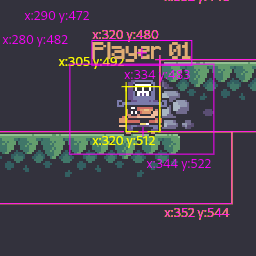
\includegraphics[width=0.5\linewidth]{assets/collisions.png}
  \caption{Collisions}
  \label{fig:collisions}
\end{figure}

\begin{figure}
  \centering
  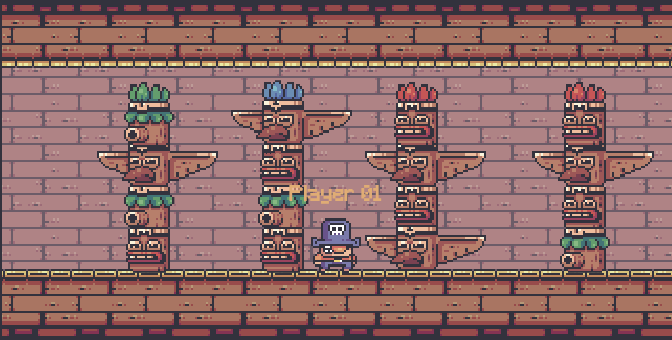
\includegraphics[width=0.5\linewidth]{assets/enemies.png}
  \caption{Enemies}
  \label{fig:enemies}
\end{figure}

\begin{figure}
  \centering
  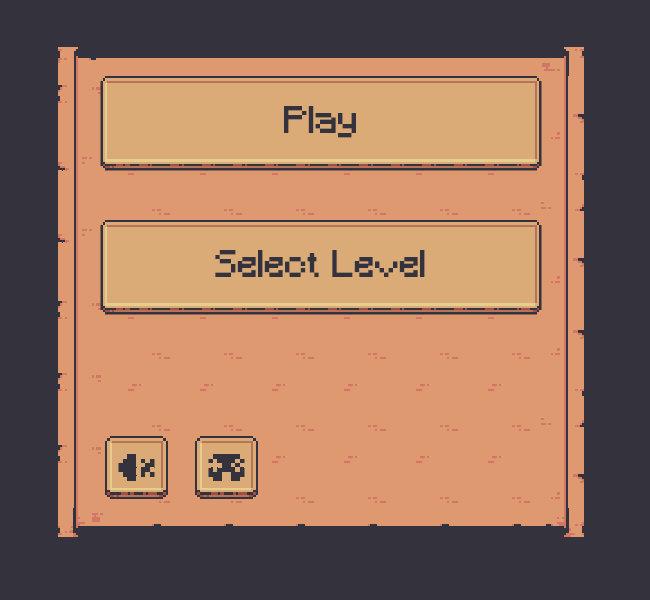
\includegraphics[width=0.5\linewidth]{assets/home.png}
  \caption{Main Menu}
  \label{fig:home}
\end{figure}

\begin{figure}
  \centering
  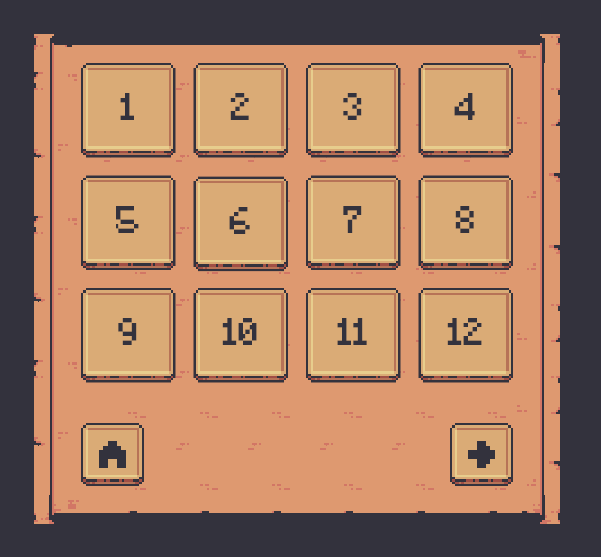
\includegraphics[width=0.45\linewidth]{assets/levels-1.png}
  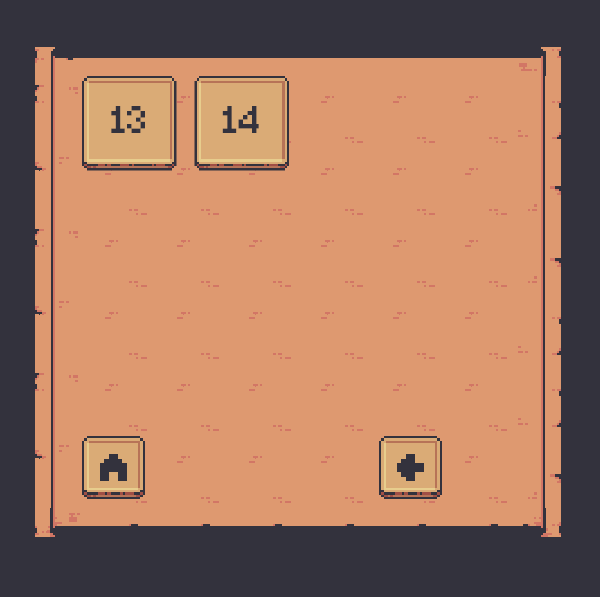
\includegraphics[width=0.45\linewidth]{assets/levels-2.png}
  \caption{Selecting Levels}
  \label{fig:levels}
\end{figure}

\begin{figure}
  \centering
  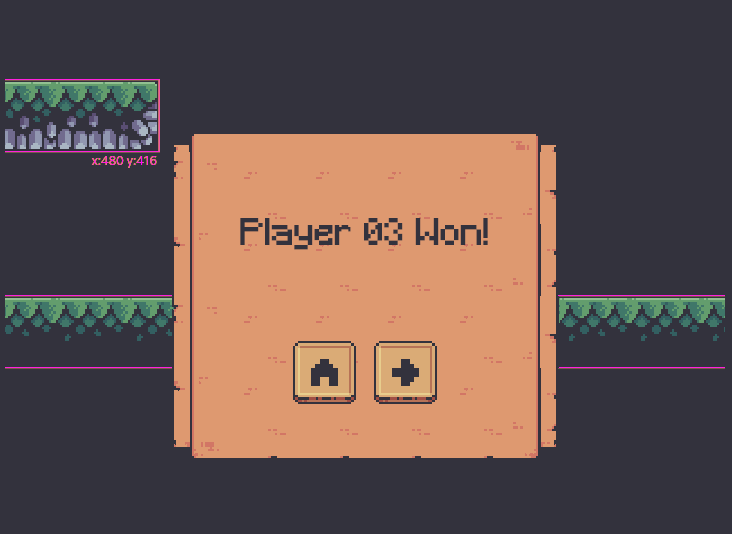
\includegraphics[width=0.5\linewidth]{assets/win.png}
  \caption{Win Prompt}
  \label{fig:win}
\end{figure}

\bibliography{refs}{}
\bibliographystyle{plain}

\end{document}